%%
%% This is file `mcmthesis-demo.tex',
%% generated with the docstrip utility.
%%
%% The original source files were:
%%
%% mcmthesis.dtx  (with options: `demo')
%% 
%% -----------------------------------
%% 
%% This is a generated file.
%% 
%% Copyright (C)
%%     2010 -- 2015 by Zhaoli Wang
%%     2014 -- 2016 by Liam Huang
%% 
%% This work may be distributed and/or modified under the
%% conditions of the LaTeX Project Public License, either version 1.3
%% of this license or (at your option) any later version.
%% The latest version of this license is in
%%   http://www.latex-project.org/lppl.txt
%% and version 1.3 or later is part of all distributions of LaTeX
%% version 2005/12/01 or later.
%% 
%% This work has the LPPL maintenance status `maintained'.
%% 
%% The Current Maintainer of this work is Liam Huang.
%% 
\documentclass{mcmthesis}
\mcmsetup{CTeX = false,   % 使用 CTeX 套装时,设置为 true
        tcn = 2000708, problem =D,
        sheet = true, titleinsheet = true, keywordsinsheet = true,
        titlepage =false, abstract = false}

\usepackage{palatino}
\usepackage{lipsum}
\usepackage{indentfirst}%%%%%%%%%%%%%设置首行缩进!!!
\title{Best team, best team performance }%\MCMversion
%\author{\small \href{http://www.latexstudio.net/}
 % \includegraphics[width=7cm]{mcmthesis-logo}%对应PDF中的latex studio标志
\date{\today}
\begin{document}
\begin{abstract}
Researches on team success are always eye-catching and heated-discussed. In this paper, we state our points on team strategies and success through several models.

To solve the first problem, we establish a multivariate weight evaluation complex network model (MWEN) by setting up a weight matrix through the distance between players, the number of passes, and positions. Combining the match time and players' position, MWEN model is visualized, which can directly reflect the relationship between different players on the field. Then, we calculate the degree centrality, betweenness centrality, closeness, clustering coefficient and other indicators. These parameters describe the relationship between a pair as well as the team from different perspectives in multiple scales. We also use label propagation community detection algorithm to identify the configurations of the network.


In the second problem, we define the player conversion rate, possession time, and action contribution, together with betweenness as four indicators to evaluate players’ performance. These indicators can describe the players' flexibility, the ability to control the ball, the cooperation with the players and so on. Using AHP to calculate the weight of new indicators, we get the comprehensive performance which can fairly reflect the contribution level of players. According to it, we get the rankings of Huskies players and different teams respectively. In addition, using the empirical distribution function of two situations under three outcomes, we draw the conclusion that the opponent's counter-strategy has greater influence on the outcome than the home team strategy.

For the third problem, we consider the goalkeeper, defender, midfielder and forward as the object of formulating structural strategy. Through cross analysis of various indicators of different positions, we get customized suggestions for each position. Through the sensitivity analysis of our model we find that “betweenness” is comparatively sensitive to the score, so we can get several structural strategies to improve the team's comprehensive performance.

To solve the last problem, we extend MWEN model to general team network by analogy analysis and case study. We analyze the subjective and objective factors of team performance through a case of virtual social network. Furthermore, we explain the quantitative methods of indicators and the construction methods of similar network models.

\begin{keywords}
Team performance; Group dynamics; Performance evaluation; Community detection 
\end{keywords}
\end{abstract}
\maketitle
\tableofcontents
\newpage
%%%%%%%%%%%%%%%%%%%%%%%%%%%%%%%%%%%%%%%%%%%%%%%%%%%%%%%%%%%%%%%%%%%%%%%%%%%%%%%%%%%%%%%%%%%%%%%%%
\section{Introduction}
\subsection{Problem background}
With the increasingly complex structure and problems of human society, the team composed of elites in various fields is more sought after by people than the big name alone. Also, the importance of the team is valued by an increasing number of people. Therefore, how the team use the best strategy to solve the problem quickly becomes a new exploration direction for some scholars.
One of the most informative settings to explore team processes is in competitive team sports. In this paper, we have the Huskies to be our home soccer team with their all 38 games against their 19 opponents. 
\begin{itemize}
\item To understand the team’s dynamics, we are asked to create network for the passes.
\item Then, player’s performance plays a vital role in exploring the reasons for team success. Our home soccer team and the opponents should all be taken into consideration.
\item For practical significance, we will work out the strategies for the Huskies.
\item For generalized use, not just in a controlled setting team, we should consider group dynamics and performance in various fields.
\end{itemize}
 %\lipsum[2]
%%我们的问题%%%%%%%%%%%%%%%%%%%%%%%%%%%%%%%%%%%%%%%%%%%%%%%%%%%%%%%%%%%%%%%%%%%%%%%%%%%%%%%%%%%%%%%%%%%
\subsection{Our work}
To further present our solutions, we arrange our paper as follow:
\begin{itemize}
\item In section 2 and 3, we give out the reliable assumptions to simplify the model, then the symbols listed are used to describe our model.
\item In section 4, to solve problem A, we take each player as a node, and build a complex multivariate network model to identify network patterns and properties.
\item In section 5, to solve problem B, after identify the player's and team's performance indicators, we use analytic hierarchy process to quantify the weight of indicators. Then, we do regression analysis of the Huskies' and their opponents' performance which is the comprehensive performance that can fairly reflect players' contribution, thus drawing the conclusion of team strategies.
\item In section 6, to solve problem C, we make use of Stacked Bar Chart to compare various indicators of different positions, thus get customized suggestions for each position.What's more, we do sensitivity analysis on each indicator, and then get several structrual strategies to improve team performance.
\item In section 7, to solve problem D, we generalize our model to solve team issues in various fields.
\item At last, we discuss the strenghths and weaknesses of our model in detail.

\end{itemize}
%%假设%%%%%%%%%%%%%%%%%%%%%%%%%%%%%%%%%%%%%%%%%%%%%%%%%%%%%%%%%%%%%%%%%%%%%%%%%%%%%%%%%%%%%%%%%%%%%%%%%%%%%
\section{Assumptions}
To simplify our problems, we make the following basic assumptions:
\begin{itemize}
\item Accurate and true data provied by "2020 Problem D DATA".
\item If the outgoer and receiver of two adjacent passes are the same player, the time difference between the two passes is approximately the ball possession time of the player (ignoring the ball rolling time).
\item When a player passes, the player who receives the ball is in the destination in the data we use.
\item If a shot is followed by "Reflexes" of the other side's goalkeeper, it means that the player on his own side has scored and the other side's goalkeeper has lost the ball. If not, it will be regarded as a goal failure.
\item The ID of regular players and substitute players in the same position can not be identified by playing time, and the distinction between them should be inferred in the figures.
\item All fields are the same size and shape.
\end{itemize}
%%命名法%%%%%%%%%%%%%%%%%%%%%%%%%%%%%%%%%%%%%%%%%%%%%%%%%%%%%%%%%%%%%%%%%%%%%%%%%%%%%%%%%%%%%%%%%%%%%%%%%%%
\section{Nomenclature}
In this paper we use the nomenclature in Table1 to describe our model. Other symbols that are used only once will be described later.
%表格
\begin{table}[htbp]
\centering  % 表居中
\begin{tabular}{lccc}  % {lccc} 表示各列元素对齐方式,left-l,right-r,center-c
\hline
Symbol &Significance\\ \hline  % \hline 在此行下面画一横线

$W_{ij}$ &Weight between nodes in adjacency matrix \\         
$d_{ij}$ &Distance between nodes in adjacency matrix \\ 
$C_{D}^{w\alpha}\left(i\right)$ &Improved weighted Degree of player i\\        % & 表示列的分隔线
$C_{closeness}\left(i\right)$ &Measurement of the difficulty of reaching code i \\ 
$C_{betweenness}\left(i\right)$ &Measurement of the indispensability of code i to a network\\ 
$C_{total}\left(G\right)$ & Measurement of the clustering of the whole network\\ 
$C_{performance}$ &Comprehensive performance score of player i \\
$C_{goal}\left(i\right)$ &Direct contribution score of player i \\
$C_{con}\left(i\right)$ &Conversion rate score of player i\\
$C_{possessionTime }\left(i\right)$ &Total possession time score of player i\\
$C_{action}\left(i\right)$ &Individual action contribution score of player i\\ 

\hline
\end{tabular}
\caption{Nomenclature}
\end{table}
%结束
%%模型陈述%%%%%%%%%%%%%%%%%%%%%%%%%%%%%%%%%%%%%%%%%%%%%%%%%%%%%%%%%%%%%%%%%%%%%%%%%%%%%%%%%%%%%%%%%%%%%%
\section{ Solution to Problem A }
In this section, we discuss all the details about our model used for problem A, followed by the solutions and problem-solving process.
\subsection{Data pre-processing}%数据处理
We use the "passingevent.csv" file provided by the topic to build a two-dimensional coordinate system.


We know from the data provided by the topic:
\begin{itemize}
\item There are 4 kinds of players: ’F’ forward, ‘D’ defender, ‘M’ midfielder, ‘G’ goalkeeper;  
\item A unqiue identifier for each match played during the season, and reflects the order of the match in the season;
\item MatchPeriod\\
The half in which the event took place. '1H': first half, '2H': second half;
\item EventTime\\
The time in seconds during the MatchPeriod (1st or 2nd half) at which the event took place.
\end{itemize}


By abstracting the player as a node, the position of the player, i.e., the coordinate, is determined. We assume that there are players $i$ and $j$ of the Huskies:
\begin{itemize}
\item We calculate the distance of each Huskies’ player at different time and normalize it by the position of the players' coordinates.
\item The number of passes from player $i$ to player $j$ in the table is calculated and normalized.
\item Distinguish the passing categories of different players.
\end{itemize}


\subsection{MWEN model}  %权重矩阵网络模型

We construct the MWEN model according to the weighted (adjacency) matrix:

According to Javier et al. (2012), this basic visual analysis can be more quantified by calculating global network invariants (describing the overall characteristics of a team) or local invariants (providing insight into individual participants). They all depend on the adjacency matrix $W$, where $W_{ij}$ in the matrix $W$ has a weight from player $i$ to player $j$.\\
It's not hard to know that the further away players are from each other on the pitch, the less connected they are. Similarly, the number of passes between players reflects the closeness of their relationship.


For the type of passes, consider the connection between different players’ positions. For example, the same position usually passes more passes, while the connection between different positions is usually weakened according to the farther position they usually have in the court. In addition, the model visualization we implemented finally forms a directed graph, and the possibility of player $i$ passing to player $j$ is different from that of player $j$ passing to player $i$.


Through the above rules, the following standards are established and nomalized.

\begin{figure}[h]
\small
\centering
\includegraphics[width=10cm]{criteria.png}
\end{figure}


Let the (normalized) distance be $L_{ij}$, the number of passes be $n_{ij}$, quantitative passes category index be $f_{ij}$, where $i,j\in \left\{\ F,M,D,G \right\}$
%%%传球类别的定量化指标源集合为(这里可以用画个箭头的图FMDG排成一排,标有数字的有向箭头)!!
%%公式1
\begin{eqnarray}
f_{ji}=\left\{\begin{array}{lr}
    1- f_{ij}       \qquad   f_{ij}>0.5\\
    f_{ij}          \qquad \qquad  f_{ij}=0.5\\
\frac{1}{2}\times f_{ij}   \qquad   f_{ij}<0.5\\
\end{array}
\right.\\
\end{eqnarray}
\begin{equation}
W_{ij}=\alpha\cdot \frac{1}{ L_{ij}}+\beta\cdot n_{ij}+\gamma\cdot f_{ij}
\end{equation}

According to the importance, we give 0.2, 0.4 and 0.4 weights to $\alpha$, $\beta$ and $\gamma$ respectively. Finally, we get the weight adjacency matrix $W$ of $i$ to $j$ from the above formula:
\begin{equation}
W=
\left[ \begin{array}{cccc}
('F','F') & ('F','M') & ('F','D') & ('F','G')\\
('D','D') & ('D','M') & ('D','G') & ('D','F')\\
('M','F') & ('M','M') & ('M','D') & ('M','G')\\
('G','F') & ('G','M') & ('G','D') & ('G','G')
\end{array}\right]
=\left[ \begin{array}{cccc}
1 & 0.75 & 0.5 & 0.25\\
1 & 0.75 & 0.5 & 0.5\\
0.25 & 1 & 0.25 & 0.25\\
0.25 & 0.25 & 0.5 & 0
\end{array}\right]
\end{equation}

\subsection{Dynamic model visualization} %动态模型模型可视化

Weight will be used to measure the length and thickness of different nodes in the network, and to measure the proximity between two players. 

We have mapped the visual tracks of players in the first half and the second half of all data in passingevent.csv. Space and dynamics are shown on the graph by intercepting the average positions of players in different time periods. Because it is not sure whether the player is a substitute in a match, whether he or she will play midway or not, and we use all- matches data for having more accurate results, according to the degree of correlation between the midpoint and the point in the figure, that is, the closer the same type of players get together, the more likely they are substitutes for each other, and the shape of the match can also be seen. 


Although we have the data in the range [0, 100], we reshape the following figures to the actual size of a soccer field.
\begin{figure}[h]
	\begin{minipage}[t]{0.5\textwidth}
		\centering
		\includegraphics[width=8cm]{first_half(2).jpg}
		\caption{Passing networks for the Huskies in the first half in proportion to the actual size of the soccer field, using the passingEvents data\label{fig:aa}}
	\end{minipage}
	\qquad
	\begin{minipage}[t]{0.5\textwidth}
		\centering
		\includegraphics[width=8cm]{second_half.jpg}
		\caption{Passing networks for the Huskies in the second half in proportion to the actual size of the soccer field, using the passingEvents data\label{fig:aa}}
	\end{minipage}
\end{figure}


The position of the node represents the average location of the player on the field, the size of the point represents the touch times of the player, and the color of the point represents the position of the player who passes the ball: yellow is the goalkeeper $G$, red is the forward $F$, orange is the midfielder $M$, and light yellow is the defender $D$. The point label represents the player's name. The thickness of the line represents the weight, and the color of the line represents the position of the player passing the ball.

\subsection{Identify network patterns and configurations}
\begin{itemize}
\item Network indicator
\end{itemize}

Through several local network invariants of the ball-passing network, we measure the individual contribution of a player in a team.
\begin{itemize}
\item Improved weighted Degree
\end{itemize}
Improved weighted Degree is a measure of the importance of players. Improved weighted Degree is the weight of quantity and branch chain weight, using Degree Centrality Measure proposed by Tore Opsahl et al.(2010) for reference:
\begin{equation}
C_{D-out}^{w\alpha}=k_{i}^{out}\times\left( \frac{s_{i}^{out}}{k_{i}^{out}}\right)^{\alpha}
\end{equation}
\begin{equation}
C_{D-in}^{w\alpha}=k_{i}^{in}\times\left( \frac{s_{i}^{in}}{k_{i}^{in}}\right)^{\alpha}
\end{equation}
\begin{equation}
C_{D}^{w\alpha}=\frac{C_{D-in}^{w\alpha}+C_{D-out}^{w\alpha}}{2}
\end{equation}


where $\alpha$ is a positive tuning parameter that can set according to the research setting and data.We set$\alpha$0.8 here referring to literature. If this parameter is between 0 and 1, then having a high degree is taken as favorable, whereas if it is set above 1, a low degree is favorable. $k^{out}$ represented the activity of a node, that is, the number of ties that originate from a node. $k^{in}$  shows the number of ties that are directed towards a node, a proxy of its popularity. $s^{out}$ and $s^{in}$ are defined as the total weight attached to the outgoing and incoming ties, respectively. $C_{D}$ is the degree of one node.

\begin{itemize}
\item Closeness
\end{itemize}
Direct measurement of the difficulty of reaching a specific player in a team(using Python package):
\begin{equation}
C_{closeness}\left(i\right)=\frac{1}{\sum\limits_{j}d_{ij}}
\end{equation}

where $d_{ij}$ is defined as the distance between two nodes:
\begin{equation}
d_{ij}=\frac{1}{w_{ij}}
\end{equation}
where $w_{ij}$ is the weight between node $i$ and $j$.

\begin{itemize}
\item Betweenness
\end{itemize}
\begin{equation}
C_{betweenness}\left(i\right)=\sum_{j\neq k\neq i}\frac{n_{jk}}{g_{jk}}
\end{equation}

where $n_{jk}$ is the number of nodes on the shortest path through node $i$, and $g_{jk}$ is the number of nodes on the path between $j$ and $k$ through node $i$.
\begin{itemize}
\item Global clustering coefficient
\end{itemize}
In graph theory, clustering coefficient is a measure of the degree to which points in a graph tend to cluster together. The evidence shows that in most real networks and special social networks, nodes have a strong tendency to form a group, which is characterized by a relatively close connection.


The global clustering coefficient measures the clustering of the whole network, based on the triple of nodes. A triple is one of three nodes with two (open triples) or three (closed triples) undirected edge connections. A triangle consists of three closed triples, which are concentrated on each node. The global aggregation coefficient is the number of closed triples in all triples (both open and closed).

\begin{equation}
C_{total}\left(G\right)=\frac{3\times G_{\Delta}}{3\times G_{\Delta}+G_{\bigwedge}}
\end{equation}
where $G_{\Delta}$ represents the number of closed triples in the path; $G_{\bigwedge}$ represents the number of open triples in the path.

\begin{itemize}
\item Local clustering coefficient
\end{itemize}
\begin{equation}
C_{i}=\frac{2|\left\{e_{jk}\right\}|}{u_{i}\left(u_{i}-1\right)}
\end{equation}

where $|\left\{e_{jk}\right\}| $represents the $\textbf{the number of connections}$ between its adjacent nodes, and $\frac{u_{i}\left(u_{i}-1\right)}{2}$represents $ \textbf{the number of all possible connections}$ between adjacent nodes.

The clustering coefficient of the whole network 
$\overline{C}=\sum\limits_{i}C_{i}$
can also be defined by Watts and Strogatz as the mean value of the local clustering coefficient of all nodes $n$.

\subsubsection{Network configuration}
Network dyadic and triadic configurations is a popular community detection problem. Here, Through "asyn lpa communities" algorithms in Python (ASYN), we repeatedly set the label of a node to be the label that appears most frequently among that nodes neighbors until each node has the label that appears most frequently among its neighbors. Results are as follows:

\begin{table}[htbp]%表格!!!
\linespread{1.5}
\centering
\begin{tabular}{|c|c|c|c|c|c|} 

\hline
 \multicolumn{4}{|c|}{Community Detection Results of Huskies Team}\\ 
\hline 
& \multicolumn{4}{|c|}{}& \\
& \multicolumn{4}{|c|}{D2,D4,D5,D6,D7,D8,} & G1\\ 

M12 &\multicolumn{4}{|c|}{F1,F2,F3,F4,F5,F6,}&D1,D10,\\

& \multicolumn{4}{|c|}{M1,M10,M11,M13,M2,M3,M4,} &D3,D9\\ 

& \multicolumn{4}{|c|}{M5,M6,M7,M8,M9} &\\ 
\hline 
\end{tabular}
\caption{Community Detection Results of Huskies Team}
\end{table}

Because of the randomness of the community detection algorithm results, it can be seen from the representative community results (Table 2) that four defenders and a goalkeeper are a community, which has set up the huskies team's back line and become a more reasonable community, while the forward and the midfield do not constitute a dyadic or triadic configuration, which shows that the whole team cooperates tacitly. So the network is team configuration.


It is worth mentioning that we found that the results of the community based on the self-defined weight matrix are not good. The results shown above are only based on the number of passes as the weight index. Although it looks unitary, from another perspective, it shows that a single index considering only the number of passes is conducive to the simplest and direct reflection of the community structure. But, this does not mean that our weight algorithm is redundant. Compared with ASYN algorithm only considering the number of communities, in fact, MWEN model takes more indicators into consideration, which can comprehensively reflect the performance of team members and is relatively more stable. Therefore, we will continue to use MWEN model in following parts.


\subsection{Structural indicators and network properties}
By calculating the Improved weighted Degree, Closeness, Betweenness, Global clustering coefficient and Local clustering coefficient of different types of players, we can get the values of the pair's indicators and the four types of indicators of the whole team in one game and the whole season, and figures.


Then, we consider the differences of Degree, Closeness, Betweenness, and Clustering between two players. Using 350s of a game as a time interval to include enough passes, we select the two players with the highest betweenness value in an intense game, and continuously observe the changes of betweenness value of the two players in different time intervals. Because there are not enough data, the index is almost zero in different periods of time. Therefore, in a single game, we set the index value as $index_i$ for the pair ,and set $index_{total}=\frac{\sum_{i} index_{i}}{n}$  for the whole team, which is the average value of all nodes.


We multiply different indicators by coefficients, so that they fall roughly in the same two-level range, which is convenient for observation and analysis at the same time.

\begin{figure}[h]
	\begin{minipage}[t]{0.5\textwidth}
		\centering
		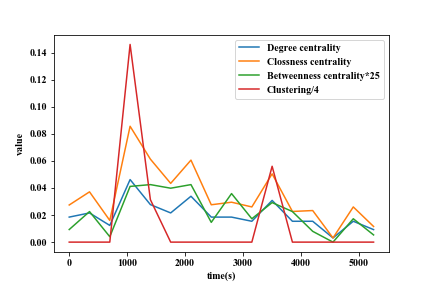
\includegraphics[width=7cm]{value_of_graph_per_game_2_players.png}
		\caption{Two players in one game\label{fig:aa}}
	\end{minipage}
	\qquad
	\begin{minipage}[t]{0.5\textwidth}
		\centering
		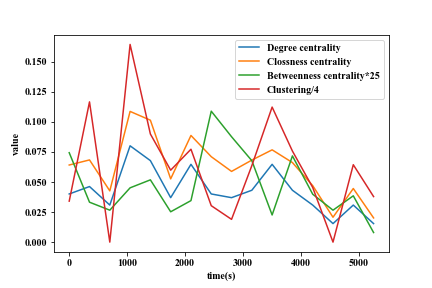
\includegraphics[width=7cm]{value_of_graph_per_game.png}
		\caption{Whole team in one game\label{fig:aa}}
	\end{minipage}
\end{figure}

As shown in Figure 3, for 2 players, Clustering fluctuates greatly with time in one game and has lots of 0 values, while Betweenness, Closeness and Degree tend to be more stable in a certain range, where Closeness has the largest average value, followed by Degree and Betweenness, showing that this pair are close to each other in the game. What's more, players are more energetic in the first half of the game because the value of four indicators goes down over time. In Figure 4, for the whole team, Betweenness and Clustering fluctuate greatly, which indicates players often change their formation. Compared with them, the other two indicators have similar vibration amplitudes and respective average values, showing the team's close connection.


For the whole season, we use the same method to segment each game, and draw the changes of different indicators of the fixed two nodes in different games, that is, the changes of different indicators of the whole team with the game number.
The figures are as follows.


\begin{figure}[h]
	\begin{minipage}[t]{0.5\textwidth}
		\centering
		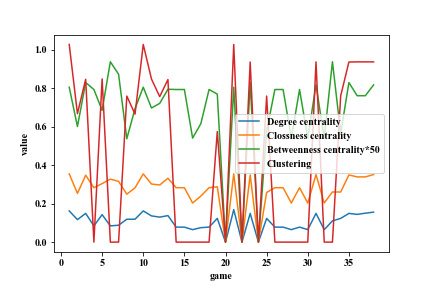
\includegraphics[width=7cm]{value_of_graph_one_season_2_players.png}
		\caption{Two players in one season\label{fig:aa}}
	\end{minipage}
	\qquad
	\begin{minipage}[t]{0.5\textwidth}
		\centering
		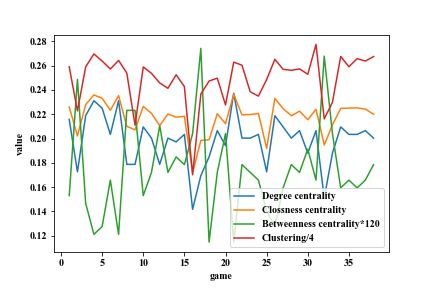
\includegraphics[width=7cm]{value_of_graph_one_season.png}
		\caption{Whole team in one season\label{fig:aa}}
	\end{minipage}
\end{figure}

As shown in Figure 5, for 2 players, Clustering fluctuates frequently and greatly over the season, while Betweenness, Closeness and Degree tend to be more stable in a certain range, where Closeness has the largest average value, followed by Degree, then by Betweenness, which illustrates that players tend to act similarly in each game, except their formation. At the same time, in Figure 6, for the whole team, Betweenness fluctuates greatly. Compared with it, the other three have similar vibration amplitudes and respective average values,showing the similar formation.

\section{ Solution to Problem B }
The performance of players has a significant influence on many aspects, such as team strategy, player rankings, and player compensation. How to describe players' performance quantitatively has become more and more vital for coaches. A player's performance is related to many factors, such as, ratio of goals per shot, possession in genral, possession characteristics, smart passes and so on.

\subsection{Data pre-processing}%数据处理
The "fullevents.csv" data of players with opponents adds information such as soccer moves and shots. Using these added information, we can not only identify the football movement,thus grading each player's performance, but also identify the substitute's playing time. Moreover, the time when the team scored the goal and other information can be clarified as well. It is conducive to our better analysis of player's performance with these information.

\subsection{Quantify performance index}
\begin{equation}
C_{performance}= C_{direct}+ C_{indirect}
\end{equation}


Because player's personal performance is not only related to whether he scores goals thus leading to the direct result of the game, but also closely related to whether he reasonably cooperates with his teammates, responds to cover and helps teammates score. Therefore, we divide player's contribution into direct and indirect score contribution.


\subsubsection{Direct score contribution }
Designate direct score contribution as $C_{goal}$.
\begin{equation}
C_{goal}=f(R)=e^{a_{0}\cdot R+b_{0}}
\end{equation} 

Goal proportion is:
\begin{equation}
R =\frac{n_{goal} }{n_{shot}},
\end{equation}


where ${n_{shot}$ is the total number of shots a player has in a game. Goal scoring can be measured by the number of shot actions of the player, minus the number of defensive failures of the other team, i.e., the number of reflexes of the other goalkeeper. It should be noted that only forwards and centers may have direct score contribution.

\subsubsection{Indirect score contribution}
Indirect score contribution can be defined as follows:
\begin{equation}
C_{indirect }=\alpha2\beta2\cdot C_{ con }+\alpha3\beta3\cdot C_{ possessionTime }+\alpha4\beta4\cdot C_{ Betweenness }+ \alpha5\beta5\cdot C_{action}
\end{equation}


where $\alpha_{i}$ is weight, $\beta_{i}$ is dimensional correction factor.

We use AHP to determine the above parameters.
Consistent judgement matrix
Denote $\left\{x_{1}, x_{2}, x_{3}, x_{4}\right\} as \left\{ C_{betweenness}, C_{action}, C_{possesion}, C_{possessionTime}\right\}$.From the matrix proposed by Saaty, we get the following pairwise comparison matrix $M$ :

\begin{equation}
M=
\left[ \begin{array}{cccc}
1 & 5 &3 & 7 \\ 
1/5 & 1 & 3/5 & 3/7 \\
1/3 & 5/3 & 1 & 7/5 \\
1/7 & 7/3 & 7 & 1 \end{array}\right]
\end{equation}

After calculation, we get CI= 0.04502561010707584, CR= 0.04020143759560343\textless0.1

Compared with matrix $W$ , we pass the consistence test and get the weight vector
 $(\alpha_{2},\alpha_{3},\alpha_{4},\alpha_{5})=(0.6052347,0.08969842,0.17162574,0.13344114)$



\begin{itemize}
\item Player conversion rate score (Possesion charge score)
\end{itemize}

The calculation of player conversion rate score is that each time the Huskies get the ball from their team member, pass it to the next player on their own side and get one point, until it reaches the player in the other team, then two points will be reduced. At this time, a conversion rate scoring period ended, and the next conversion rate scoring period starts from the next time the Huskies get the ball.Tthe total conversion rate of players is the cumulative score of all scoring periods.
\begin{equation}
C_{con}=\sum\limits_{i}^{n}C_{ con }^{i}
\end{equation}

\begin{itemize}
\item Total possession time score
\end{itemize}
The calculation method is from the time when the Huskies get the ball as the destiny player to the time when the Huskies pass it to their opponents. This time period is the scoring period of one ball control time. Then the total possession time is the sum of the one ball control time.
\begin{equation}
C_{possessionTime }=\sum\limits_{i}^{n}C_{ possessionTime}^{i}
\end{equation}

\begin{itemize}
\item Betweenness score
\end{itemize}
As mentioned in the previous chapter, being an important parameter from the network model, betweenness is defined as the central media ability of the player and other players, which represents the indispensable degree of the player in the whole team i.e., if the player is substituted, the team's passing chain will be disconnected a lot or completely. Therefore, this indicator can also be used as a standard to measure indirect contribution.

\begin{itemize}
\item Individual (event)action contribution score
\end{itemize}
The action of players also has a great impact on the game. A player's good action, such as a smart pass and a clearance, can help the team to control the ball and win a score, while a bad action, such as a foul, may lead to his being sent off, thus making the team lose its original stable formation. Therefore, according to the knowledge of football, we can define the individual action contribution score of players through their actions. The formula is as follows:
\begin{equation}
\begin{array}{lr}C_{action}= 4 \cdot Ground attacking duel  + 4 \cdot Ground defending duel +1\cdot Ground loose ball duel\\
+3\cdot air duel +1\cdot launch +3\cdot clearance +5\cdot smart pass +2\cdot cross -2\cdot kick cross
\\ -7\cdot fuel+3\cdot Acceleration
+1\cdot Goalkeeper leaving line -10\cdot Out of game foul\\ +3\cdot Save attempt -8\cdot other fuel -5\cdot Reflexes
\end{array}
\end{equation}


where ground attacking duel, ground defending duel, ground loose ball duel, air duel, launch, clearance, smartpass, cross, acceleration, goalkeeper leaving line, save attempt are regarded as the action that contributes to the team's score, and its contribution rate weight is given according to relevant information and empirical evidence. However, fuel, kick cross, out of game foul are regarded as fouls of different degrees, which can reduce players' scores. For "the other fuel" given in the table, we always give the weight of "-8" for the sake of simplification. In addition, reflexes refers to defensive failure, which represents the negative contribution rate of the defensive players.


In addition, it should be noted that for different positions, there will be their own regular actions. For example, in the indicator calculation, the midfield usually takes the task of shot, while the goalkeeper rarely passes and takes more defensive actions. Therefore, for each player, when we consider all the action indicators, we can evaluate their performance comprehensively and fairly.


Finally, the comprehensive indicator of players' performance $C_{performance}$ is obtained by summing up each indicator.

\begin{equation}
\begin{array}{lr}C_{performance}=C_{direct}+ C_{indirect}\\
= \alpha1\beta1\cdot C_{goal }+ \alpha2\beta2\cdot C_{ trans }+\alpha3\beta3\cdot C_{ controltime }+\alpha4\beta4\cdot C_{ Betweenness }\\
+ \alpha5\beta5\cdot C_{action}\\
\end{array}
\end{equation}

After establishing all performance indicators above, we have the Huskies rankings and all teams' rankings, shown the performance of each team and every single player. 

\begin{figure}[h]
	\begin{minipage}[t]{0.5\textwidth}
		\centering
		\includegraphics[width=8cm]{rankings.png}
		\caption{The Huskies rankings \label{fig:aa}}
	\end{minipage}
	\qquad
	\begin{minipage}[t]{0.5\textwidth}
		\centering
		\includegraphics[width=8cm]{teamrank.png}
		\caption{Rankings of all teams \label{fig:aa}}
	\end{minipage}
\end{figure}



To analyze the influence of the performance indicators we proposed, on one hand, we pick out two players from the Huskies and their opponents, respectively. Then we compare the performance indicators of them and display them by radar chart.

\begin{figure}[h]
\small
\centering
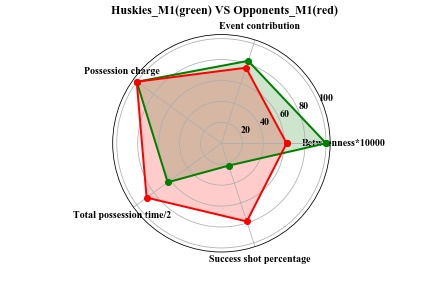
\includegraphics[width=9cm]{dota_radar.jpg}
\caption{Huskies M1 VS Opponents M1} \label{fig:aa}
\end{figure}

As is depicted in the chart, both player have a high conversion rate score i.e., possesion charge score, showing their close contact with their team members and being a great midfield. It is obvious that Huskies M1 is an integral part of the team, while Opponents M1 has weaker influence. However, Opponents M1's success shot percentage is much higher than Huskies M1, and total possession time is higher than Huskies M1, which means Opponents M1 is a briliant contributor to team scoring. Event contribution has rarely different effect on the two players' success. 

On the other hand, the top 11 players who have the best scores under four indicators: Betweenness, Event contribution, Total possesion time and conversion rate were taken into consideration to analyze the Huskies and the change of the average index of all opponents, i.e., the overall level of the specific indicators of European team members. For each indicator, we select the top 11 players in the team, that is to say, the ID of the players under each indicator is not necessarily the same. However, due to the ranking of indicators from high to low, this image shows the distribution level of different indicators in players in an ingenious way.


\begin{figure}[h]
	\begin{minipage}[t]{0.5\textwidth}
		\centering
		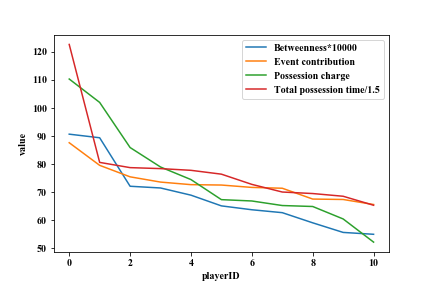
\includegraphics[width=8cm]{value_of_person_per_season_Huskies.png}
		\caption{Top 11 players of The Huskies \label{fig:aa}}
	\end{minipage}
	\qquad
	\begin{minipage}[t]{0.5\textwidth}
		\centering
		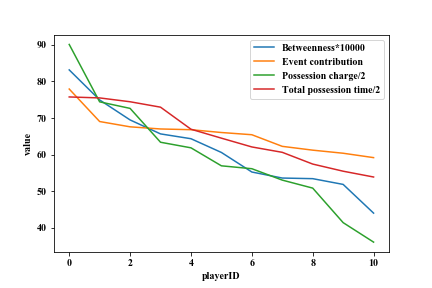
\includegraphics[width=8cm]{value_of_person_per_season_Opponents.png}
		\caption{Top 11 players of the Opponents\label{fig:aa}}
	\end{minipage}
\end{figure}

As shown in Figure 8, the distribution of indicators shows a smooth exponential distribution, that is, most players' indicators are relatively concentrated, while the best few players' indicators are far ahead. The higher the ranking is, the greater the difference of the index value of the adjacent ranking is. Meanwhile, we can draw a conclusion from Figure 9 that the vast majority of the opponents' indicators are at average level, and few players have relatively high indicators.


In addition, we compare the Huskies and one of the opponents' performance.

\begin{figure}[h]
	\begin{minipage}[t]{0.5\textwidth}
		\centering
		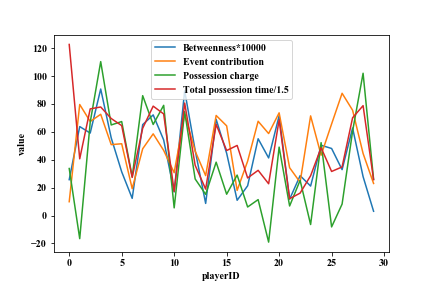
\includegraphics[width=8cm]{value_of_player_per_season_Huskies_30player.png}
		\caption{30 players of The Huskies \label{fig:aa}}
	\end{minipage}
	\qquad
	\begin{minipage}[t]{0.5\textwidth}
		\centering
		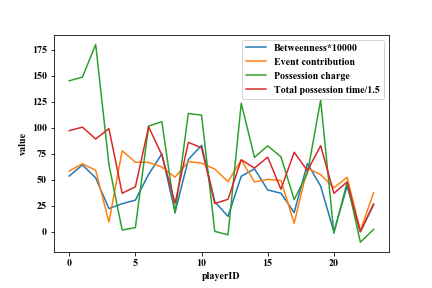
\includegraphics[width=8cm]{value_of_player_per_season_Opponents_24player.png}
		\caption{24 players of the Opponents\label{fig:aa}}
	\end{minipage}
\end{figure}


In Figure 10, we can have a thorough view of the Huskies performance. It is shown that some of the players have high balanced indicators, such as, ID 12 and 20, while ID 5, 10 and 13 have relatively weak performance. In addition, most of the Huskies have their own strengths and weaknesses, so the team should develop in a balanced way. We can evaluate the opponents' performance through Figure 11, among which the ID 8 and 21 are relatively balanced but the overall value is low, most of the other players have different indicator values.

\subsubsection{Strategy universality}

A good decision can make the team score more goals in all competitions, but it can also depend on the capability of the enemy team. Meanwhile, we assume that a good strategy is to improve the team's own comprehensive strength, that is, a good strategy represents a higher team performance score. 

Here, we have obtained the comprehensive performance scores of each team in each game. According to this, we consider the impact of our team's performance score on the number of goals of our team. In addition, we consider the impact of the difference between our team's performance score and the other team's performance score on goals, i.e., we also consider the other party's strength. 

\begin{euquation}
C_{performance}^{diff}= C_{performance}^{Huskies}- C_{performance}^{opponent}
\end{euquation}

We assume that when the team wins the game, the performance score of the team is generally higher, but when the team loses the game, the score is generally lower(Jordi Duch, 2010). Performance scores may present different distribution levels under different competition results. Therefore, we consider drawing the performance of the host team and the performance difference between the host team and other teams according to the results of the three kinds of competitions: loss, win and tie.\\


The experience distribution function of $C_{performance}$, $C_{performance}^{diff}$ under different competition results is shown in the figure. We find out that the shape of empirical distribution function is similar and separated from each other, and it has a very normal geometry.

We use the exponential function to adjust the parameter of $y=\frac{1}{(1+exp^{-c*(x-d)})}$,

and make regression analysis. The result shows that the regression is very good.

\begin{figure}[h]
	\begin{minipage}[t]{0.5\textwidth}
		\centering
		\includegraphics[width=8cm]{fittingC.png}
		\caption{Empirical distribution function and fitting line of C_{performance} \label{fig:aa}}
	\end{minipage}
	\qquad
	\begin{minipage}[t]{0.5\textwidth}
		\centering
		\includegraphics[width=8cm]{fittingCdiffer.png}
		\caption{Empirical distribution function and fitting line of C_{performance}^{diff}\label{fig:aa}}
	\end{minipage}
\end{figure}

For the figure of $C_{performance}$, we look at the value of 50, and it can be seen that the probability of performance score on the right side of the value is 0.6, 0.52 and 0.3, respectively. Hence, there is a positive correlation between performance score and winning situation.

For the figure $C_{performance}^{diff}$, the distribution difference of the three curves is greater than above. Take point 0 as an example, the probability of $C_{performance}^{diff}$ on the right side of the value is 0.8, 0.5 and 0.2, respectively, which shows that the distribution difference of $C_{performance}^{diff}$ is more significant under different winning and losing levels. In other words, the value of $C_{performance}^{diff}$ is more significant for the outcome.

By comparison, we can see that the team's winning and losing results are positively correlated with the team's $C_{performance}$ and $C_{performance}^{diff}$, but the latter has a stronger impact on the outcome. Therefore, we come to the conclusion that the strategy has certain effect, but it depends on the opponent's counter-strategy more.


\section{Solution to Problem C}

\subsection{Cross Analysis}
In fact, it is difficult to study and formulate a team's structural strategy through the network model with low risk of uncertainty because the ball passing network of a team in a football match changes with time and space, and when one makes his own actions, others will make corresponding responses at the same time, i.e., the network has many uncertainty. Hence, we analyze the specific positions one by one, consider their improvement, and give the optimal strategy for each position in the network.

There are forward, midfielder, defender and goalkeeper in the team. They play different main roles, including goalkeeper opposing other team from scoring, defender tackling, midfielder assisting attack and shooting, forward mainly shooting, which forms a stable structure in the match field.

Based on the data from the previous calculation, we draw a stacked histogram of the players' indicators. Among them, we put players of the same profession adjacent to each other in order to learn the strengths and weaknesses of each position from the figure.

\begin{figure}[h]
\small
\centering
\includegraphics[width=10cm]{stacked.png}
\caption{Four indicators' score of all players} \label{fig:aa}
\end{figure}

The positions are goalkeeper, defense, forward, midfield from left to right.

\begin{itemize}
\item Goalkeeper 

As is depicted from the figure, goalkeeper's betweenness and possession charge scores are at average level, but has low event contribution score, which means he should improve the skill to prevent the opposing team from scoring and perform smart goal kicks. Compared with the average level of the whole team, the goalkeeper has more time to hold the ball, which shows that the goalkeeper's ability to control the ball is  great.

\item Defense

The defenders' indicators are at a high level. More betweenness and possession time show that the defenders of the team have a strong ability to stabilize the rear, to control the field, and to tackle. A close relationship between the defenders is conducive to driving the whole team's attack and defense. The high conversion rate score indicates that the guard's passing is more flexible, and a good contribution rate of movement also shows that the rear tailgate is their good personal skill. All in all, almost all defenders' indicators have reached a quite satisfactory standard, except D10 defender who has low scores in all aspects.


\item Forward

The overall ability of forwards is not as good as that of midfielders, and their betweenness is at the average level. For possession charge, there are great differences between different players, which shows that the flexibility of the forward team is uneven, so it is necessary to enhance the passing training among the players.


\item Midfield

The midfielder accounts for nearly half of the team, however, their betweenness scores differ at relatively low level. Player M1, M3, M4, M6, M9, M13, have a quite great ability of passing ball, while others are far below average. It is speculated that these should be substitute players, which may be that they have not been well trained. Therefore, it is necessary to appropriately increase the opportunities for substitute players to be trained. Anyhow, the overall skill of midfielders still needs to be strengthened. We can consider learning relevant experience with the defenders to enhance the defense ability
\end{itemize}

Through the stacked histogram, we clearly show the indicators of different team members and even the indicators of the team. Through analysis above, we get the improvement strategies for each position, so as to effectively improve the overall performance level of the team.


\subsection{Sensitivity Analysis}

\resizebox{\textwidth}{22mm}{
\begin{tabular}{|c|c|c|c|c|c|c|c|} 
\hline
&Betweenness&Event contribution&Possession charge&Total possession time&Changing proportion&Average score&Deviation of score\\
\hline
0&0.60523
&0.08970
&0.17163
&0.13344
&0\%
&42.0180
&0.00\%
\\
\hline
1&0.69602
&0.08970
&0.17163
&0.13344
&15\%
&45.9827
&9.31\%
\\
\hline
2&0.51445
&0.08970
&0.17163
&0.13344
&-15\%
&38.1073
&-9.31\%
\\
\hline
3&0.60523
&0.10315
&0.17163
&0.13344
&15\%
&42.7107
&1.65\%
\\
\hline
4&0.60523
&0.07624
&0.17163
&0.13344
&-15\%
&41.3253
&-1.65\%
\\
\hline
5&0.60523
&0.08970
&0.19737
&0.13344
&15\%
&42.9642
&2.25\%
\\
\hline
6&0.60523
&0.08970
&0.14588
&0.13344
&-15\%
&41.0717
&-2.25\%
\\
\hline
7&0.60523
&0.08970
&0.17163
&0.15346
&15\%
&42.7710
&1.79\%
\\
\hline
8&0.60523
&0.08970
&0.17163
&0.11342
&-15\%
&41.2649
&-1.79\%
\\
\hline
\end{tabular}}


As for the advice on the coach, we consider our several performance scores the main factor contributing to team success, and access their impact on team success by sensitivity analysis.
The table above showed our results. We set each indicator a 15\% deviation and -15\%deviation in turn and observe the final performance score’s alteration.  It’s easy to know that 15\% change in betweenness results in 9\% change in total event contribution, while the same changing proportion of event contribution, possession charge, total possession time cause 1.6\%,2.3\%,1.8\% change in final performance score respectively.

Therefore, we identify the betweenness has largest impact on team success.
Next, we put forward several suggestions to improve players’ betweenness. First, increase players training time properly and target at efficient coordination in passing patterns. Second, put more importance on players’ assistance to each other to strengthen the bound. Thirdly, forcing players to interact with who have good possession of ball. Last but not least, promote everyone to participant in real match.

\section{Solution to Problem D}
After analyzing the group dynamics in a controlled setting of a team sports, generalizing the findings is also worth being emphasized. As indispensable as social network is, we explore the indicators that social network team performance has on the basis of comprehensive consideration. Through the analysis, we think there are the following points to consider. First of all, we divide the impact into subjective factors and objective factors. Subjective factors often represent more complex interpersonal relationships between people, while objective factors affect the performance level of the whole team from the physical function of people and the overall scale of the team.

\begin{figure}[h]
\small
\centering
\includegraphics[width=10cm]{processplot.png}
\caption{Team performance factors} \label{fig:aa}
\end{figure}

\subsection{Objective factors}
\begin{enumerate}
\item Education level

The education level of the team members determines the working efficiency of the team, to a great extent. Especially in the field of high technology, the academic certificate of team members shows their knowledge range and comprehensive quality. In addition, professional level and additional skills are also a bonus for team work.

%\begin{itemize}
\item Wage level
%\end{itemize}

Salary level, including the welfare and vacation of players, can be regarded as an incentive measure for employees. Well paid teams usually have high enthusiasm and subjective initiative for work, which is consistent with the evaluation indicators of our above-mentioned network model of ball passing.

%\begin{itemize}
\item External characteristic
%\end{itemize}

The external objective characteristics of the team, such as age and gender distribution of the team, usually play a crucial role in the team success. Young team members are often the fresh blood in the team, while the old are well-experienced. The appropriate gender ratio is powerful for the harmony and stability of the team.
\end{enumerate}
\subsection{Subjective factors}
\begin{enumerate}
\item Communication

Team members' communication ability is an important factor to maximize internal information. The number of communication between team members reflects the work intensity and cooperation density of the team, which is conducive to the overall performance improvement of the team. 


\item Coordination

The difference between cooperation and communication between team members is that the latter pays more attention to the idea exchange efficiency of specific tasks, while the former only summarizes the frequency of contact between players in general. The good cooperation of team members not only improves the tacit understanding and efficiency of the team, but also creates a comfortable working atmosphere.

\item Relationship building

Intimacy reflects the cohesion of a team member and the consolidation of the relationship. The lack of trust between individuals in a team may lead to fierce infighting, which will greatly reduce the team's performance level. Face to face interaction, personal phone, etc. can reflect the intimacy between team members.


\item Leadership

The management personnel in the team can make an indispensable contribution to the overall planning of the whole team. The management ability of the leader can unify the team objectives, establish a hierarchical team structure, and thus improve the efficiency of the team. In addition, leadership is also conducive to improving the fairness of the team and solving the disputes among the team members.
\end{enumerate}

\subsection{Case analysis}
\indent Chong King Tan et al.(2018) had a quite thorough research of the social network. They considered several indicators influencing team performance in the virtual social network. Here, we can make an analogy to the virtual social network, using the complex multivariate network model of ball passing and other indicators.

\indent Accordingly, the number of emails and other important information sent and received, and the positions of employees in the team reflect the important position of employees in the social network of the virtual company. We consider using the number of e-mails sent and received between team members and the average time spent on work communication on social platform to quantify communication ability indicators. In addition, the distribution of cultural sources of team members also affects the work efficiency of team members.


\section{Strengths and weaknesses}
Our complex multivariate network model has following strengths and weaknesses.
\subsection{Strengths}
\begin{itemize}
\item The model makes full use of the data given, and establishes a time-space dynamic network model of the ball passing, which can well reflect the internal mechanism of players' relation and realize the visualization of time and space.
\item Combined with the actual situation of football field, the model analyzes the meaning and function of various actions, and defines some new indicators, such as the flexibility between players, the ability of possession, closeness, as well as the score of players' action contribution rate, which can reflect players' comprehensive indicators comprehensively.
\item Owing to our clear logic, the model and figures are intuitive so that we can get all kinds of players' information, which is helpful for decision makers to make decisions.
\item The model can be generalized, as is shown in the last problem, that is to say, how to apply the model to the evaluation of social networks is well illustrated.
\item The model not only uses precise parameters, but also adds the impact of various factors, so that the stability of the model increases. Therefore, the calculation results obtained in use can well fit the actual situation.
\end{itemize}




\subsection{Weaknesses}
\begin{itemize}
\item In fact, in order to simplify the model, we still have some imperfections. For example, although we can infer the information of the substitute through the data, we do not clearly separate the player and the substitute in the image displayed, which is also because the data we process is relatively large.
\item Although many researches have proved that the traditional clustering method can achieve community detection, the results we make by clustering have some unsatisfactory. Due to time constraints, we need to make further improvement according to the model.
\end{itemize}%\lipsum[6]


%\lipsum[9]

\section{Conclusions}
In this paper, firstly, based on improved weighted matrices, we establish a complex multivariate network model of balling passes, taking each player as a node. Then, we define and calculate the node indicators in the network. Using traditional clustering methods for these indicators, we recognize the network pattern and its changes over time.


Secondly, we introduce several new indicators to evaluate the performance of soccer players, and use AHP to determine the importance weight of each new index for the performance of players, so as to get the comprehensive performance of each player and the team.

Thirdly, We make use of Stacked Bar Chart to get formulating structural strategy. We then change different indicators respectively, and make sensitivity analysis on the final score of the Huskies, thus providing the coach with team structual strategies to improve team success.

Finally, with the analogy idea, we extend the model to social network.Through case analysis, we provide the way of thinking on how to analyze network model indicators.



%%%%%%%%%%%%%%%%%%%%%%%%%%%%%%%%%%%%%%%%%%%%%%%%%%%%%%%%%%%%%%%%%%%%%%%%%%%%%%%%%%%%%%%%%%%%%%%%%%%%%%%%%%%%%%
%%这里添加参考文献%%%%%%%%%%%%%%%%%%%%%%%%%%%%%%%%%%%%%%%%%%%%%%%%%%%%%%%%%%%%%%%%%%%%%%%%%%%%%%%%%%%%%%%%%%%%
\begin{thebibliography}{99}%添加参考文献
\bibitem{1}Narizuka, Takuma, et al. "Statistical Properties of Position-Dependent Ball-Passing Networks in Football Games." Physica A: Statistical Mechanics and Its Applications, vol. 412, 2014, pp. 157–168., doi:10.1016/j.physa.2014.06.037.
\bibitem{2}Opsahl, Tore, et al. "Node Centrality in Weighted Networks: Generalizing Degree and Shortest Paths." Social Networks, vol. 32, no. 3, 2010, pp. 245–251., doi:10.1016/j.socnet.2010.03.006.

\bibitem{3}Javed, Muhammad Aqib, et al. "Community Detection in Networks: A Multidisciplinary Review." Journal of Network and Computer Applications, vol. 108, 2018, pp. 87–111., doi:10.1016/j.jnca.2018.02.011.
\bibitem{4}Pe˜na, Javier L´opez. "A Network Theory Analysis of Football Strategies." 2012.
\bibitem{5}Duch, Jordi, et al. "Quantifying the Performance of Individual Players in a Team Activity." PLoS ONE, vol. 5, no. 6, 2010, doi:10.1371/journal.pone.0010937.
\bibitem{6}Long, Hua, and Baoan Li. "Overlapping Community Identification Algorithm in Directed Network." Procedia Computer Science, vol. 107, 2017, pp. 527–532., doi:10.1016/j.procs.2017.03.105.
\bibitem{7}Tan, Chong King, et al. "Factors Influencing Virtual Team Performance in Malaysia." Kybernetes, vol. 48, no. 9, 2019, pp. 2065–2092., doi:10.1108/k-01-2018-0031.

\bibitem{8}Pappalardo, Luca, et al. "A Public Data Set of Spatio-Temporal Match Events in Soccer Competitions." Scientific Data, vol. 6, no. 1, 2019, doi:10.1038/s41597-019-0247-7.

\bibitem{9}Raghavan, Usha Nandini, Réka Albert, and Soundar Kumara. "Near linear time algorithm to detect community structures in large-scale networks." Physical Review E 76.3 (2007): 036106.


\end{thebibliography}
%%%%%%%%%%%%%%%%%%%%%%%%%%%%%%%%%%%%%%%%%%%%%%%%%%%%%%%%%%%%%%%%%%%%%%%%%%%%%%%%%%%%%%%%%%%%%%%%%%%%%%%%%%%%%
\begin{appendices}%添加代码文件

\section{Appendix}

 %\lipsum[13]

The solution to the four questions about the model \\

 \textcolor[rgb]{0.98,0.00,0.00}{\textbf{Question one:}}
\lstinputlisting[language=Python]{./code/TTTTT.py}

%%%%%%%%%%%%%%%%%%%%%%%%%%%%%%%%%%%%%%%%%%%%%%%%%%%%%%%%%%%%%%%%%%%%%%%%%%%%%%%%%%%%%%%%%%%%%%%%%%%%%%%%%%%%
\end{appendices}
\end{document}

%% 
%% This work consists of these files mcmthesis.dtx,
%%                                   figures/ and
%%                                   code/,
%% and the derived files             mcmthesis.cls,
%%                                   mcmthesis-demo.tex,
%%                                   README,
%%                                   LICENSE,
%%                                   mcmthesis.pdf and
%%                                   mcmthesis-demo.pdf.
%%
%% End of file `mcmthesis-demo.tex'.
